\begin{frame}{PM\tsub{2.5} Exposure Assessment}
\begin{itemize}
    \item PM\tsub{2.5} is one of most important public health concerns 
    \begin{itemize}
        \item Associated with 4.2 million deaths in 2015 (GBD, 2016) 
        \item Associated with 2.7 -- 3.4 million preterm births in 2010 (Malley et al., 2017)
    \end{itemize}
\end{itemize}
\begin{center}
    \bf \color{red} PM\tsub{2.5} Exposure $\leftrightarrow$ Ambient PM\tsub{2.5} Levels
\end{center}
\begin{figure}
    \centering
    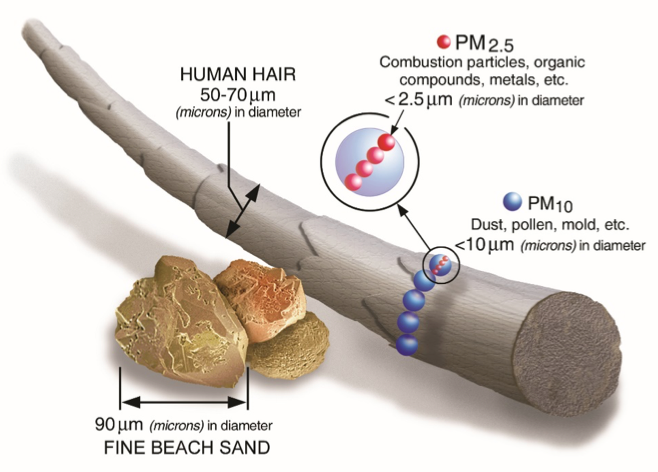
\includegraphics[width=0.5\textwidth]{img/pm25.png}
    \label{fig:pm25}
\end{figure}
\vspace{-0.4cm}
\begin{center}
    \textit{\tiny Image courtesy of U.S. EPA}
\end{center}
\end{frame}

\begin{frame}{Spatiotemporally Continuous PM\tsub{2.5} Predictions}

Satellite-based empirical model:
\vspace{-0.5cm}
\begin{center}
    \footnotesize
    \gatherblock{Ground\,PM_{2.5}\,Obs._{(s,t)} = f(AOD_{(s,t)}, Met.\,Params_{(s,t)}, LU\,Params_{(s)})}
\end{center}

\begin{itemize}
    \item Built on predictors/indicators of ground-level PM\tsub{2.5}
    \begin{itemize}
        \item Satellite data: \textbf{Aerosol Optical Depth (AOD)}
        \item Meteorological parameters
        \item Land-use parameters
    \end{itemize}
    \item Compared to chemical transport models and dispersion models
    \begin{itemize}
        \item Higher spatial ($\leq$1 km) and temporal (daily and sub-daily) resolutions
        \item Higher accuracy and precision
    \end{itemize}
\end{itemize}
\begin{center}
    \color{red} Model development/performance depends on the amount and quality of \textbf{satellite AOD} and \textbf{ground PM\tsub{2.5} measurements}
\end{center}
\end{frame}

\begin{frame}{Satellite AOD Missingness}
    \begin{itemize}
        \item Non-random missing satellite AOD mainly because of cloud and snow-cover 
        \item A large proportion, $\sim$70\%, of satellite AOD retrievals are missing in the US (for the MODIS 10-km AOD products)
    \end{itemize}
    \begin{center}
    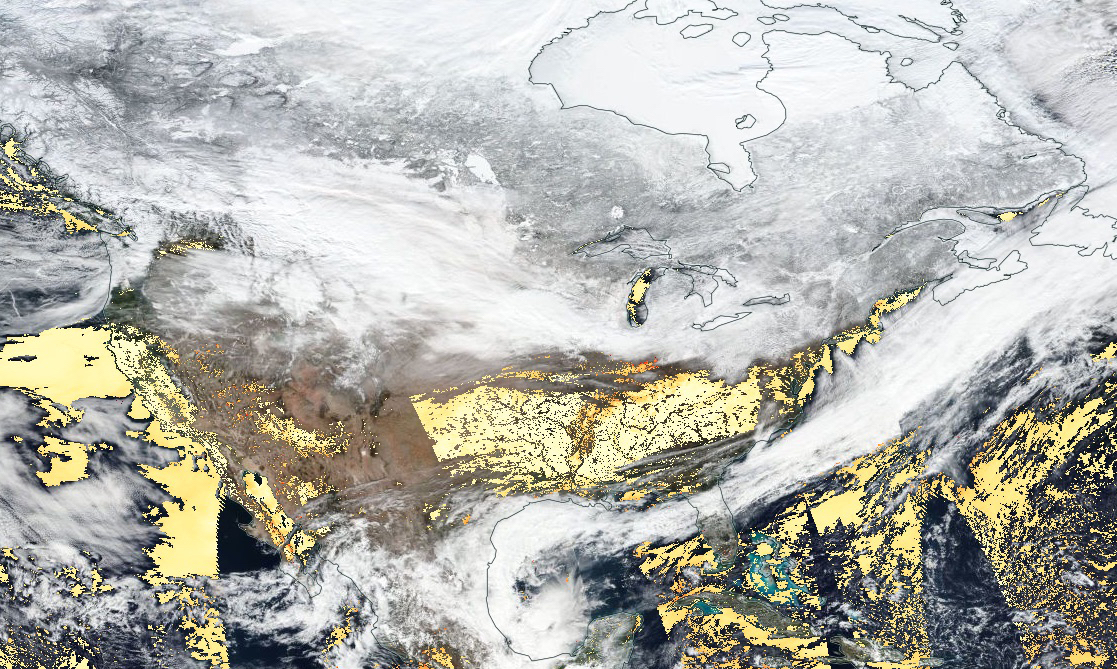
\includegraphics[width=0.6\textwidth]{img/missing.jpg} \\
    \vspace{-0.2cm}
    {\tiny Cloud and snow covers blocked satellite AOD observation (USGS EarthExplorer, 2018)}
    \end{center}
    \begin{center}
        \color{red} Estimated missing AOD data caused by cloud/snow cover
    \end{center}
\end{frame}

\begin{frame}{Regulatory Monitoring Coverage in the US}
    \begin{figure}
        \centering
        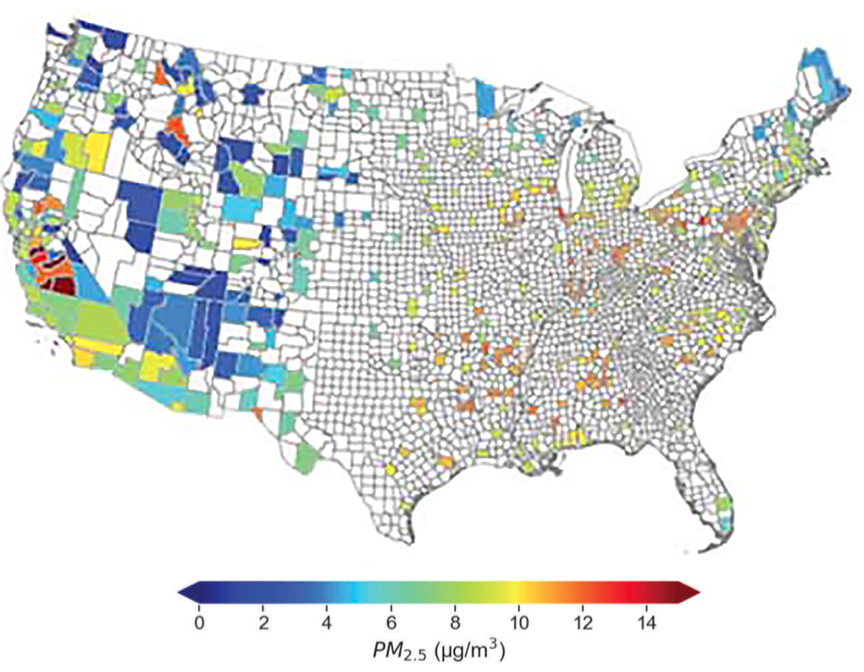
\includegraphics[width=0.7\textwidth]{img/counties.png}
        \caption{\footnotesize County-level maps of annual mean PM\tsub{2.5} in 2011 (AQS + IMPROVE)}
        \label{fig:my_label}
    \end{figure}    
    \vspace{-0.2in}
    \begin{center}
        \tiny\sl Image courtesy of Diao et al., (2019)
    \end{center}
\end{frame}

\begin{frame}{Low-Cost Sensor Data}
    \begin{itemize}
        \item \textbf{Data-poor regions: regions with insufficient ground observations and other supporting data}
        \item Low-cost air quality sensors ($<$ \$2,500) are a potential data source to fill in the gaps of regulatory air quality data  
        \item Low-cost sensor data have lower data quality
    \end{itemize}
    \begin{figure}
        \centering
        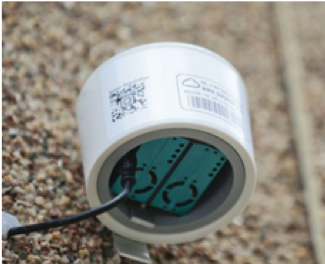
\includegraphics[height=0.25\textwidth]{img/sensor1.png} \hspace{5px}
        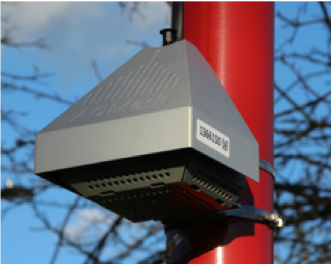
\includegraphics[height=0.25\textwidth]{img/sensor2.png} \hspace{5px}
        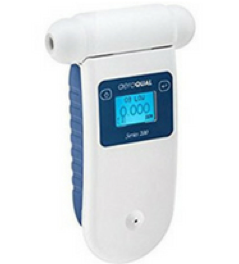
\includegraphics[height=0.25\textwidth]{img/sensor3.png}
    \end{figure}
    \begin{center}
        \color{red} Developed a weighted method to combine regulatory and low-cost sensor data
    \end{center}
\end{frame}